\documentclass[fleqn,letterpaper,12pt,printwatermark=false]{memoir}
% memoir commands to define the text block geometry
\setulmarginsandblock{0.5in}{*}{*}
\setlrmarginsandblock{0.5in}{*}{*}
% put "extra" vertical space at the bottom of a page
\raggedbottom 

\usepackage{amsmath}
\usepackage{etoolbox} % for \ifblank etc
\usepackage{xparse} % for NewDocumentCommand et al.
\usepackage{enumitem}
\usepackage{transparent} % for \transparent, which I use in the watermark
\usepackage[slantedGreek]{mathpazo} \usepackage{helvet} % use Palatino et al.
\usepackage{booktabs} % prettier tables

\usepackage[]{xwatermark}
\newwatermark*[
    allpages,
    color=red!30,angle=45,
    scale=4,
    xpos=-10, ypos=0
]{%
    \transparent{0.4}dhasan example%
}

\usepackage{dashundergaps} % for \gap
\dashundergapssetup{
    teacher-mode=true, % set to true to show answers 
    gap-format=underline,
    teacher-gap-format=underline,
    gap-font={\sffamily},
    gap-numbers=true,
    gap-widen=true,
    gap-extend-percent=150, % note: making this too big might create errors
    gap-number-format=\,\textsuperscript{\normalfont(\thegapnumber)},
}

\usepackage{tcolorbox}
\tcbuselibrary{skins}
\tcbuselibrary{raster}

\usepackage{graphicx}
\graphicspath{ {../images/} }
\begin{document}

\newcommand{\myClassName}{Pre-AP Algebra 2}
\newcommand{\myUnitNumber}{1}
\newcommand{\myUnitTitle}{Introduction to Functions}
\newcommand{\myLessonNumber}{2}
\newcommand{\myLessonTitle}{Attributes of Relations and Functions}


\copypagestyle{myPagestyle}{empty}


\newcommand{\myFooterSize}{\footnotesize}
\makeoddfoot{myPagestyle}{{}}{\myFooterSize{\thepage{}~of~\pageref*{xwmlastpage}}}{\myFooterSize\thetitle}
\makeevenfoot{myPagestyle}{{}}{\myFooterSize{\thepage{}~of~\pageref*{xwmlastpage}}}{\myFooterSize\thetitle}

%
% A command to change the appearance of the cognitive verb 
% in the objectives.
%
\newcommand{\myCognitiveVerb}[1]{\textcolor{blue}{\textbf{#1}}}

%
% Terminology explanation:
%
% "unit" refers to the Algebra 2 unit being taught.
% "section" refers to the section within the unit being taught.
% "heading" refers to the headings in this document (Objectives, Example, ...)
%
\NewDocumentCommand{\myUnitSectionNumberFont}{}{\sffamily\bfseries\HUGE}
\NewDocumentCommand{\myUnitNameFont}{}{\sffamily\large}
\NewDocumentCommand{\mySectionNameFont}{}{\sffamily\bfseries\huge}
\NewDocumentCommand{\myHeadingFont}{}{\sffamily\bfseries\Large}


%
% #1 is the fill-in text
%
\NewDocumentCommand{\myFillInBlank}{m}{%
    \,%
    \gap[u]{#1}%
    \,%
}


% Definition for the LESSON HEADER + OBJECTIVES
%
% #1 : optional unit name
% #2 : optional unit/section number
% #3 : mandatory title
%
\NewDocumentEnvironment{myNotesHeader}{oom}{
    \title{#3}
    \begin{flushleft}
        \IfValueT{#2}{{\myUnitSectionNumberFont#2}}
        \hfill\;\;
        \begin{minipage}[b]{0.75\textwidth}
            \begin{flushright}
                \IfValueT{#1}{
                    {\myUnitNameFont#1}\\ \vspace{0.75em}
                }
                {\mySectionNameFont#3}
            \end{flushright}
        \end{minipage}
        \hrule
    \end{flushleft}
    \noindent{\myHeadingFont Objectives:}
    \begin{enumerate}[label=\arabic*)]
}{
    \end{enumerate}
}


% Definitions related to the VOCABULARY TABLE
%
\newenvironment{myVocabulary}{
    {\noindent{\myHeadingFont Vocabulary:}}\vspace{1em}

    \begin{tabular}{ll}
        \toprule
            \emph{word} & \emph{meaning} \\ 
        \midrule
}{
    \bottomrule
    \end{tabular}
    \vspace{1em}
}

\newcommand{\myVocabularyWord}[2]{%
{\textcolor{blue}{\textbf{#1}}} & #2 \\
}


% Definitions related to an INTRODUCTION
%
\newenvironment{myIntroduction}{
    {\noindent{\myHeadingFont Introduction:}}\vspace{1em}

    \setlength{\leftskip}{3cm}
}{
    \setlength{\leftskip}{0pt}
}


% Definition related to KEY CONCEPTS
%
% #1 : the key concept (which appears as a tcolorbox title)
%
\NewDocumentEnvironment{myKeyConcepts}{ O{Key Concepts:} }{
    \begin{tcolorbox}[
        title=#1, fonttitle=\myHeadingFont,
        coltitle=black, 
        colbacktitle=black!25!yellow, 
        colframe=black!50!yellow,
        colback=white!70!yellow,
        boxrule=2pt, 
        ]
}{
    \end{tcolorbox}
}


% Definition related to EXAMPLES
%
% #1 Optional example number 
% #2 A statement of the example problem.
% #3 How much empty vertical space to leave for the example box.
%
\NewDocumentCommand{\myExample}{omm}{%
    \begin{tcolorbox}[
        enhanced,
        sharp corners, 
        colback=white,
        boxrule=0pt,
        borderline={0.5pt}{0pt}{black,dashed},
        ]
        {\myHeadingFont Example\IfValueT{#1}{{ #1}}:}
        #2
        \tcblower
        \vspace{#3}
    \end{tcolorbox}
}

% Definitions related to PROBLEMS

% A counter to number the problems in the guided notes.
\newcounter{MyProblemCounter}
\setcounter{MyProblemCounter}{1}
\newcommand{\useMyProblemCounter}{\theMyProblemCounter\stepcounter{MyProblemCounter}}

% an environment for two adjacent problems
%
% #1 : directions for all the problems
% #2 : vertical height of the problem boxes
% #3 : details for problem 1
% #4 : details for problem 2
%
\newenvironment{myProblems2}[4]{%
    \noindent
    {\myHeadingFont Practice:}\hspace{0.5em}#1\nopagebreak%
    \begin{tcbraster}[%
        raster equal height,%
        raster columns=2,%
        raster column skip=0.5mm,%
        raster row skip=0.5mm,%
        raster every box/.style={%
            enhanced,%
            sharp corners,%
            colback=white,%
            coltitle=black, colbacktitle=black!10!white,%
            boxrule=0pt, borderline={0.5pt}{0pt}{black},%
            title={\texttt\useMyProblemCounter},%
            },%
        ]%
        \begin{tcolorbox}[attach boxed title to top left]
            #3
            \tcblower\vspace{#2}
        \end{tcolorbox}
        \begin{tcolorbox}[attach boxed title to top right]
            #4
            \tcblower
        \end{tcolorbox}%
}{%
    \end{tcbraster}
}

% an environment for 4 adjacent problems
%
% #1 : directions for all the problems
% #2 : vertical height of the problem boxes
% #3 : details for problem 1
% #4 : details for problem 2
% #5 : details for problem 3
% #6 : details for problem 4
%
\newenvironment{myProblems4}[6]{%
    \noindent
    \textbf{\myHeadingFont Practice:}\hspace{0.5em}#1\nopagebreak%
    \begin{tcbraster}[%
        raster equal height,%
        raster columns=2,%
        raster column skip=0.5mm,%
        raster row skip=0.5mm,%
        raster every box/.style={%
            enhanced,%
            sharp corners,%
            colback=white,%
            coltitle=black, colbacktitle=black!10!white,%
            boxrule=0pt, borderline={0.5pt}{0pt}{black},%
            title={\texttt\useMyProblemCounter},%
            },%
        ]%
        \begin{tcolorbox}[attach boxed title to top left]
            #3
            \tcblower\vspace{#2}
        \end{tcolorbox}
        \begin{tcolorbox}[attach boxed title to top right]
            #4
            \tcblower
        \end{tcolorbox}%
        \begin{tcolorbox}[attach boxed title to bottom left]
            #5
            \tcblower
        \end{tcolorbox}%
        \begin{tcolorbox}[attach boxed title to bottom right]
            #6
            \tcblower
        \end{tcolorbox}%
}{%
    \end{tcbraster}
}
\pagestyle{myPagestyle}

\checkandfixthelayout
\setlist{labelindent=\parindent,leftmargin=*,itemsep=0.025em,label=$\circ$}

% ---------------------HEADER------------------------------
\begin{myNotesHeader}
    \item \myCognitiveVerb{find} the domain and range of a function
    \item \myCognitiveVerb{identify} the maximum and minimum points on a graph
    \item \myCognitiveVerb{identify} $x$- and $y$-intercepts on a graph
\end{myNotesHeader}

\begin{myVocabulary}
        \myVocabularyWord{domain}
        {
            the set of all the inputs in a relation 
            (usually $x$'s)
        }
        \myVocabularyWord{range}
        {
            the set of all the outputs in a relation 
            (usually $y$'s)
        }
        \myVocabularyWord{discrete relation}
        {
            a relation that is a bunch of separate points
        }
        \myVocabularyWord{continuous}
        {
            a relation that can be graphed as a smooth line or curve
        }
        \myVocabularyWord{intercept}
        {
            where a curve crosses the $x$- or $y$-axis
        }
        \myVocabularyWord{minimum}
        {
            the smallest $y$ value of a relation (the $y$ coordinate of the lowest point)
        }
        \myVocabularyWord{maximum}
        {
            the largest $y$ value of a relation (the $y$ coordinate of the highest point)
        }
\end{myVocabulary}

% ---------------------LESSON 1------------------------------
\begin{myLesson}[][]
    Continuous relations have \emph{infinitely many} points.
    So it's impossible to describe the relation as a set of ordered pairs, since you would have 
    to write down an infinite number of pairs.
    Similarly, we cannot write the domain or range as sets of ordered pairs.
    We need a different way to do it.
\end{myLesson}

% ---------------------CONCEPT 1------------------------------
\begin{myKeyConcepts}[To find the domain of a continuous relation\dots]
    Follow these steps:
    \setlist{labelindent=\parindent,}
    \begin{enumerate}
        \item {\bfseries\itshape Look} closely at the curve.
        \item {\bfseries\itshape Ask yourself} \,``What are the $x$ coordinates of the points on the curve?''
        \item {\bfseries\itshape Describe} those $x$ coordinates as you go from left to right.
    \end{enumerate}
    That description is the domain.
    Mathematicians use \emph{inequalities} or \emph{interval notation} in their descriptions.
    You will learn this in the examples.
\end{myKeyConcepts}

\myExample{
    Find the domain of this relation.
    \begin{center}
        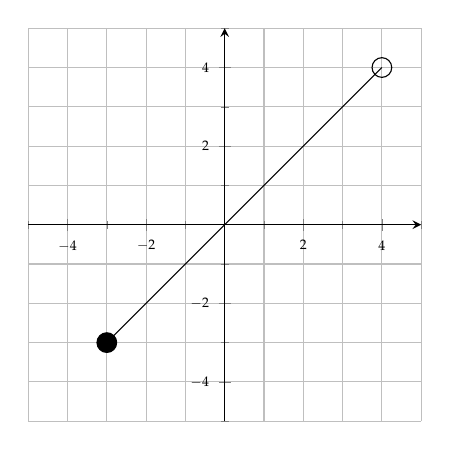
\begin{tikzpicture}
            \begin{axis}[
                width=3in,
                grid=both,
                axis x line = middle,axis y line = middle,
                axis equal image,
                xtick distance = 2, ytick distance = 2, 
                minor tick num = 1,
                xmin = -5, xmax=5,
                ymin = -5, ymax=5,
                tick label style = {font=\tiny},
                ]
                \addplot[mark=*,mark size=0.125cm,] coordinates { (-3,-3) };
                \addplot[mark=o,mark size=0.125cm,] coordinates { (4,4) };
                \addplot[no marks, samples=100, domain=-3:4, ] expression { x };
            \end{axis}
        \end{tikzpicture}
    \end{center}
}{2in}

\myExample{
    Find the domain of this relation. (The curve keeps on going forever off the grid.)
    \begin{center}
        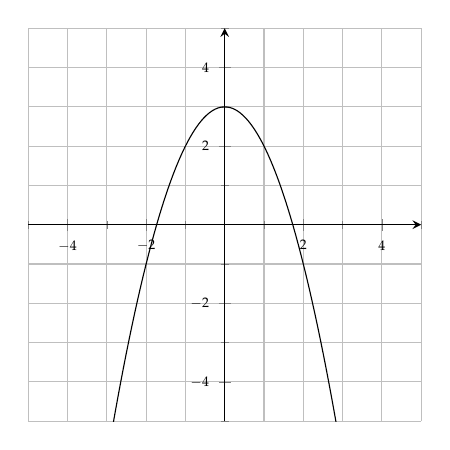
\begin{tikzpicture}
            \begin{axis}[
                width=3in,
                grid=both,
                axis x line = middle,axis y line = middle,
                axis equal image,
                xtick distance = 2, ytick distance = 2, 
                minor tick num = 1,
                xmin = -5, xmax=5,
                ymin = -5, ymax=5,
                tick label style = {font=\tiny},
                ]
                \addplot[no marks, samples=100, domain=-3:4, ] expression { -x^2 + 3 };
            \end{axis}
        \end{tikzpicture}
    \end{center}
}{2in}

% ---------------------LESSON 2------------------------------
\begin{myLesson}[][2]
    You know what intercepts are.
    They are where a graph of a function crosses the $x$- and $y$-axes.
    So if you are given the graph of a function,
    all you need to do to find the intercepts 
    is look at the graph to see where the curve crosses the axes.
    \begin{itemize}
        \item In some cases, you can see {\bfseries\itshape exactly} where it crosses
        if everything lines up nicely with the $x$-$y$ grid.
        \item But even if the curve doesn't cross the axes 
        an a point on the grid, you could still {\bfseries\itshape estimate} where 
        the crossing points are.
    \end{itemize}
\end{myLesson}

% ---------------------CONCEPT 2------------------------------
\begin{myKeyConcepts}[To find the $x$- and $y$-intercepts given the graph of a relation\dots]
    Follow these steps:
    \setlist{labelindent=\parindent,}
    \begin{enumerate}
        \item {\bfseries\itshape Draw} a dot everywhere the curve crosses either axis.
        \item {\bfseries\itshape Find} the ($x$,$y$) coordinates of those dots.
        \item The {\bfseries\itshape $x$-intercepts} are the dots on the $x$-axis.
        You may write the intercept either as the point $(x,0)$ 
        or just as the $x$ value.
        \item The {\bfseries\itshape $y$-intercepts} are the dots on the $y$-axis.
        You may write the intercept either as the point $(0,y)$ 
        or just as the $y$ value.
    \end{enumerate}
\end{myKeyConcepts}

\myExample{
    Find the $x$- and $y$-intercepts of this relation.
    \begin{center}
        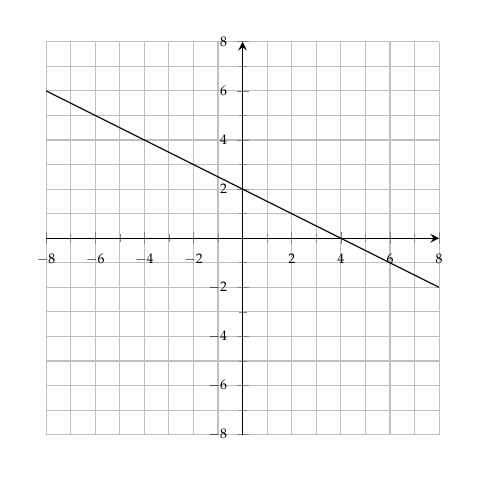
\begin{tikzpicture}
            \begin{axis}[
                width=3in,
                grid=both,
                axis x line = middle,axis y line = middle,
                axis equal image,
                xtick distance = 2, ytick distance = 2, 
                minor tick num = 1,
                xmin = -8, xmax=8,
                ymin = -8, ymax=8,
                tick label style = {font=\tiny},
                ]
                \addplot[no marks, samples=3, domain=-8:8, ] expression { -(1/2)*x + 2 };
            \end{axis}
        \end{tikzpicture}
    \end{center}
}{2in}

\myExample{
    Find the $x$- and $y$-intercepts of this relation.
    \begin{center}
        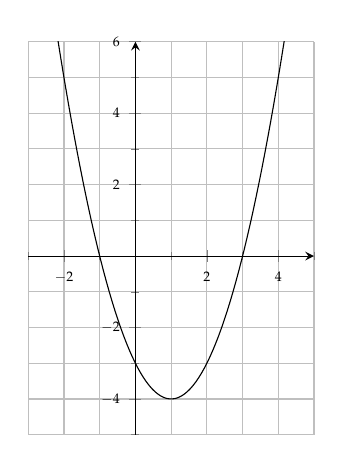
\begin{tikzpicture}
            \begin{axis}[
                width=3in,
                grid=both,
                axis x line = middle,axis y line = middle,
                axis equal image,
                xtick distance = 2, ytick distance = 2, 
                minor tick num = 1,
                xmin = -3, xmax=5,
                ymin = -5, ymax=6,
                tick label style = {font=\tiny},
                ]
                \addplot[no marks, samples=100, domain=-3:5, ] expression { (x-1)^2 - 4 };
            \end{axis}
        \end{tikzpicture}
    \end{center}
}{2in} 

% ---------------------LESSON 3------------------------------
% ---------------------CONCEPT 3------------------------------
\begin{myKeyConcepts}[To find the maximum and minimum given the graph of a relation\dots]
    Follow these steps:
    \setlist{labelindent=\parindent,}
    \begin{enumerate}
        \item {\bfseries\itshape Draw} dots on the highest and lowest points on the curve.
        \item {\bfseries\itshape Find} the $y$ coordinates of those points.
        \item The {\bfseries\itshape maximum} is the $y$ coordinate of the highest point.
        \item The {\bfseries\itshape minimum} is the $y$ coordinate of the lowest point.
    \end{enumerate}
\end{myKeyConcepts}

\myExample{
    Find the maximum and minimum of this relation.
    (The curve keeps on going forever off the top of the grid.)
    \begin{center}
        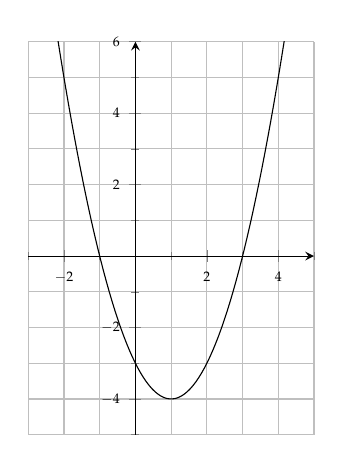
\begin{tikzpicture}
            \begin{axis}[
                width=3in,
                grid=both,
                axis x line = middle,axis y line = middle,
                axis equal image,
                xtick distance = 2, ytick distance = 2, 
                minor tick num = 1,
                xmin = -3, xmax=5,
                ymin = -5, ymax=6,
                tick label style = {font=\tiny},
                ]
                \addplot[no marks, samples=100, domain=-3:5, ] expression { (x-1)^2 - 4 };
            \end{axis}
        \end{tikzpicture}
    \end{center}
}{1.5in}

\myExample{
    Find the maximum and minimum of this relation.
    (The curve keeps on going forever off the bottom of the grid.)
    \begin{center}
        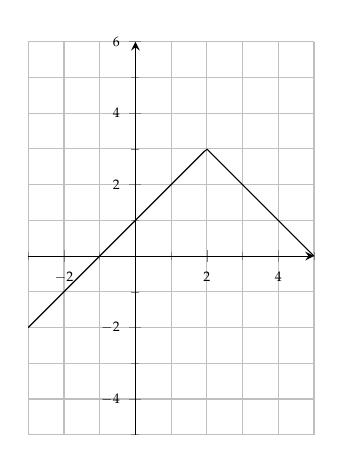
\begin{tikzpicture}
            \begin{axis}[
                width=3in,
                grid=both,
                axis x line = middle,axis y line = middle,
                axis equal image,
                xtick distance = 2, ytick distance = 2, 
                minor tick num = 1,
                xmin = -3, xmax=5,
                ymin = -5, ymax=6,
                tick label style = {font=\tiny},
                ]
                \addplot[no marks, samples=100, domain=-3:5, ] expression { -abs(x-2) +3 };
            \end{axis}
        \end{tikzpicture}
    \end{center}
}{1.5in}

% \begin{myProblems2}%
%     {Factor the following monomials into prime factors.}%
%     {2in}%
%     %
%     {\( 32x^2 \)}
%     {\( 8 x^3y^2z \)}
% \end{myProblems2}
  


\end{document}